\subsection{Calori specifici per i gas ideali}
Nei gas ideali, a seguito di evidenze sperimentali, si ha che $u = u(T)$, ovvero l'\textbf{energia interna dipende solo dalla temperatura}. Inoltre anche siccome $h = u + PV$ e $Pv = R^*T$, otteniamo che $h = h(T)$.
Quindi $c_V$ e $c_P$ sono dipendenti solo dalla temperatura e si ha che
\begin{align*}
    \text{A pressione cost.} &\qquad c_P = c_P(T) = \qty(\dv{h}{T})\\
    \text{A volume cost.} &\qquad c_V = c_V(T) = \qty(\dv{u}{T})
\end{align*}

\textbf{Relazione di Mayer}
\[ c_P = \dv{h}{T} = \frac{\dd{u} + \dd{\qty(Pv)}}{\dd{T}} = \qty(\dv{u}{T}) + \dv{R^*T}{T} = c_v + R^* \]

\subsection{Calori specifici per un gas perfetto}
Per i gas \textbf{perfetti} (gas ideali per variazioni di temperatura non troppo elevate) i calori specifici non dipendono neanche dalla temperatura:

{\renewcommand\arraystretch{1.4}
\begin{tabular}{lcc}
    \toprule
    & $c_v$ & $c_p$ \\ \midrule
    Gas Monoatomico & $\frac{3}{2}R^*$ & $\frac{5}{2}R^*$ \\
    Gas Biatomico o Poliatomico lineare & $\frac{5}{2}R^*$ & $\frac{7}{2}R^*$ \\
    Gas Poliatomico non lineare & $\frac{6}{2}R^*$ & $\frac{8}{2}R^*$ \\
    \bottomrule
\end{tabular}}

\begin{tabular}{ll}
    Monoatomico & \ch{He}, \ch{Ar}, $\ldots$ \\
    Linare & \ch{O2}, \ch{N2}, \ch{H2}, \ch{CO2}, $\ldots$ \\
    Non lineare & \ch{CH4}, \ch{H2O}, $\ldots$ \\
\end{tabular}

\subsection{Calori specifici per i liquidi}

Liquido incomprimibile ideale $C_v = C_P = c(T)$.

Liquido incomprimibile perfetto $C_v = C_P = \text{cost}$.

\subsection{Politropiche}
Trasformazione quasi statica per un sistema con un \textbf{gas ideale} dove $c_x = \text{cost}$.

Si definisce indice della politropica il temrine $n = \frac{c_x-c_P}{c_x-c_V}$

\[
    Pv^n = \text{cost} \quad Tv^{n-1} = \text{cost} \quad \frac{T^n}{P^{n-1}} = \text{cost} \quad PT^{\frac{n}{1-n}} = \text{cost}
\]

\begin{tabular}{lcc}
    \toprule
    Trasformazione & $c_x$ & $n = \frac{c_x-c_P}{c_x-c_V}$ \\
    \midrule
    Isoterma & $\pm\infty$ & 1 \\
    Isocora & $c_v$ & $\pm\infty$ \\
    Isobara & $c_P$ & 0 \\
    Adiabatica & 0 & $k = \frac{c_p}{c_v}$ \\
    \bottomrule
\end{tabular}

Per $n \ne 1$ (quindi non isoterma) l'integrale del lavoro diventa:
\begin{align*}
    l^\sra = \int_1^2 P\dd{v} &= \frac{P_1v_1}{n-1} \qty[1-\qty(\frac{v_1}{v_2})^{n-1}] \\
    &= \frac{P_1v_1}{n-1} \qty[1-\qty(\frac{P_2}{P_1})^{\frac{n-1}{n}}]
\end{align*}
Per $n = 1$ (quindi isoterma) l'integrale del lavoro diventa:
\[ l^\sra = \int_1^2 P\dd{v} = P_1v_1\ln{\frac{v_2}{v_1}} = P_1v_1\ln{\frac{P_1}{P_2}} \]

\begin{center}
    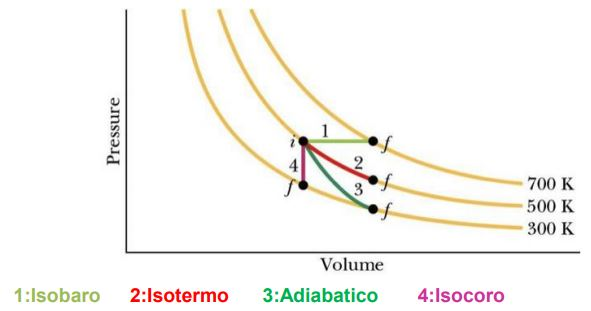
\includegraphics[height=3cm]{politropiche.JPG}
\end{center}

\subsection{Diagramma T-s}

\begin{center}
    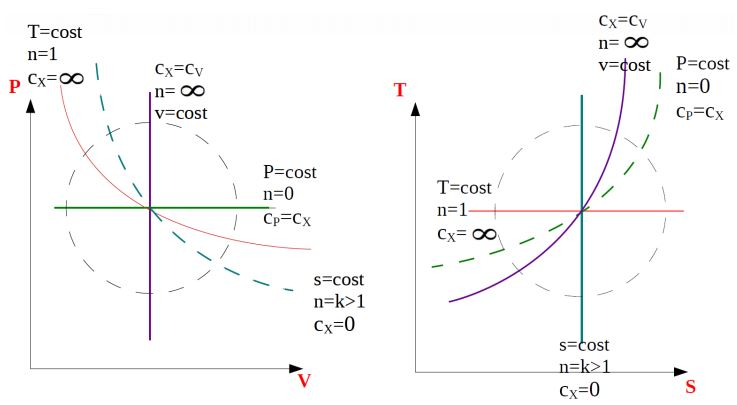
\includegraphics[height=3cm]{politropiche2.JPG}
\end{center}

L'area sottesa dalla curva in una trasformazione \emph{internamente reversibile} è uguale al calore scambiato dal sistema nella trasformazione:
\[ \dd{S}_{rev} = \frac{\dd{Q}_{rev}}{T} \qquad Q_{rev} = \int_i^f \dd{Q}_{rev} = \int_i^f T(S) \dd{S} \]

Nel piano T-s tutte le trasformazioni politropiche sono esponenziali:
\[T = T_0 e ^ { \frac{s-s_0}{c_x} }\]

\begin{tabular}{ll}
    Isoterme  (Isoentalpiche con gas ideali) & rette orizzontali \\
    Adiabatiche reversibili (isoentropiche) & rette verticale \\
    Isocore ($c_v < c_P$) & più ripide delle isobare \\
\end{tabular}

\subsection{Calcolo delle grandezze termodinamiche}
\subsubsection{Per i gas perfetti}
\begin{tabular}{lll}
    \toprule
    Trasf. intern. reversibile & $l=\int P\dd{v}$ & $q = \int \dd{q}$ \\
    \midrule
    $P = \text{cost}$ & $P\Delta v$ & $c_p\Delta T$ \\
    $v = \text{cost}$ & 0 & $c_v\Delta T$ \\
    $T = \text{cost}$ & $R^*T\ln{\frac{v_2}{v_1}} =$ & $R^*T\ln{\frac{v_2}{v_1}} =$ \\
    & $-R^*T\ln{\frac{P_2}{P_1}}$ & $-R^*T\ln{\frac{P_2}{P_1}}$ \\
    $\dd{Q}=0$ & $-c_v\Delta T$ & 0 \\
    $c_x = \text{cost}$ & $(c_x-c_v)\Delta T$ & $c_x\Delta T$ \\
    \bottomrule
\end{tabular}

\[ \Delta u = c_v \Delta T \qquad \Delta h = c_p \Delta T \]
\begin{align*}
    \Delta s &= c_v \ln{\frac{T_2}{T_1}} + R^*\ln{\frac{v_2}{v_1}} \\
    &= c_p \ln{\frac{T_2}{T_1}} - R^*\ln{\frac{P_2}{P_1}} \\
    &= c_p \ln{\frac{v_2}{v_1}} + c_v\ln{\frac{P_2}{P_1}} \\
\end{align*}

\subsubsection{Per i liquidi incomprimibili}

Se perfetti ($v =$ cost):

\[ \Delta u = c \Delta T \qquad \Delta s = c \ln{\frac{T_2}{T_1}} \]

Se ideali $c_p = c(T)$, $\beta = 0$ e $K_T = 0$:
\[ \dd{h} = c(T)\dd{T} + v\dd{P} \qquad \dd{s} = c(T)\frac{\dd{T}}{T} \]

Se perfetti:
\[ \Delta h = c\Delta T + v \Delta P \]
